\chapter{Les systèmes multi-agents}

Nous souhaitons modéliser un écosystème marin, où chaque espèce marine peut donc interagir avec une ou plusieurs autres, en fonction de ses paramètres. Si nous modélisons l'écosystème d'un point de vue programmation, nos espèces sont des objets interagissant les uns avec les autres par des méthodes, afin de pouvoir obtenir un comportement.
\\
Mais, il est beaucoup plus intéressant de pouvoir laisser ces espèces décider par eux-mêmes quel comportement adopter, pour une certaine configuration de l'écosystème à un temps \textit{t}.
\\
C'est ce qui nous a permis de nous pencher sur une branche de l'intelligence artificielle dite "distribuée", où l'intelligence artificielle est répartie sur un nombre défini d'entités, appelée "systèmes multi-agents".

\section{Qu'est-ce-qu'un "système multi-agents"?}

Les systèmes multi-agents (SMA) permettent de simuler et modéliser des comportements d'individus, appelés "agents", interagissant dans un certain environnement que l'on définira comme un écosystème\nocite{SMA}.
\\
Utilisés principalement dans la recherche en intelligence artificielle, ou combinés avec d'autres domaines scientifiques tels que la chimie ou encore la biologie, les SMA sont aussi très utilisés dans l'industrie (comme le Cinéma - pour la représentation des mouvements de foule - et dans le Jeu-Vidéo par exemple) ou encore la finance (le suivi des cours de la bourse en \textit{trading}).
\\
Afin de simuler les agents et leurs comportements, il est nécessaire (dans un souci d'efficacité et réutilisation d'outils pré-existants) d'avoir une plateforme bien spécifique à l'application que l'on souhaite faire, et au domaine associé. De nombreuses existent et se spécialisent dans différents domaines d'application. Pour notre projet, il a été décidé d'utiliser la plateforme de simulation \textbf{Netlogo}\footnote{Voir ici : \url{https://ccl.northwestern.edu/netlogo/}}, avec l'extension IODA.

\section{Présentation de la plateforme de simulation Netlogo et de l'extension IODA}

\subsection{Netlogo}
Netlogo\nocite{NetlogoManuel} est une plateforme de simulation libre et gratuite, créée en 1999. Programmée en Java et en Scala, elle a été influencé par le langage de programmation Logo quant au DSL\footnote{Un DSL est un langage dédié.} dont elle est pourvue. Très facile d'utilisation, elle a d'abord été conçue pour l'aide à la programmation dans l'éducation.
\\
La simulation Netlogo permet de prendre en compte différents agents (les \textit{turtles}) vivant dans un environnement composé de \textit{patchs} - typiquement, des carrés. Il est essentiel de savoir que plusieurs \textit{turtles} peuvent être disposés sur un même \textit{patch}, mais que chaque agent est placé sur un seul \textit{patch} à fois! Ainsi, sauf modification de l'utilisateur, un agent sera disposé au milieu d'un \textit{patch}, à distance $\frac{l}{2}$ (où \textit{l} est la longueur d'un côté de celui-ci).

\subsection{IODA}

IODA\footnote{IODA : \textit{Interaction-Oriented Design of Agent simulations}\nocite{IODAManuel}\nocite{jaamas2011-ioda} - voir ici : \url{http://www.lifl.fr/SMAC/projects/ioda/ioda_for_netlogo/doc/IODA-NetLogo-Documentation-v2.3.html}.} est une extension écrite en NetLogo, créée par deux membres de l'équipe SMAC de CRIStAL : Sébastien Picault et Philippe Mathieu. Son but est de simplifier un maximum le design et la réutilisation de simulations individu-centré, c'est à dire des simulations basées sur les conséquences globales résultant d'interactions locales entre les individus de la population du système.
\\
Les principes de IODA sont les suivants:
\begin{enumerate}
\item{une entité est un agent,}
\item{tout comportement est représenté par une règle (c'est à dire une interaction), et chaque règle est composée d'un déclencheur (optionnel), d'une condition ainsi que d'une action,}
\item{ces interactions sont affectées à des familles d'agents, exécutées par un moteur générique.}
\end{enumerate}
Ainsi, c'est le moteur générique IODA qui détermine quelles interactions peuvent avoir lieu lors d'un pas de temps. Voici une trace de son exécution (pour un pas de temps):
\begin{enumerate}
\item{les interactions de mises à jour (\textit{UPDATE}) réalisables sont exécutées par chaque agent donné,}
\item{puis chaque agent susceptible d'agir sur les autres choisit une interaction de la façon suivante:
\begin{enumerate}
\item{perçoit ses voisins (subissant les actions des autres agents),}
\item{filtre les cibles d'interactions qu'il peut effectuer,}
\item{évalue les déclencheurs et conditions de ces interactions,}
\item{sélectionne une des interactions réalisables (de priorité maximale),}
\item{exécute les actions correspondantes, présentes dans la déclaration de l'interaction.}
\end{enumerate}
}
\end{enumerate}

La Figure \ref{fig:moteur_ioda_explications} sert d'exemple quant au fonctionnement du moteur IODA.

\begin{figure}[h]
\begin{center}
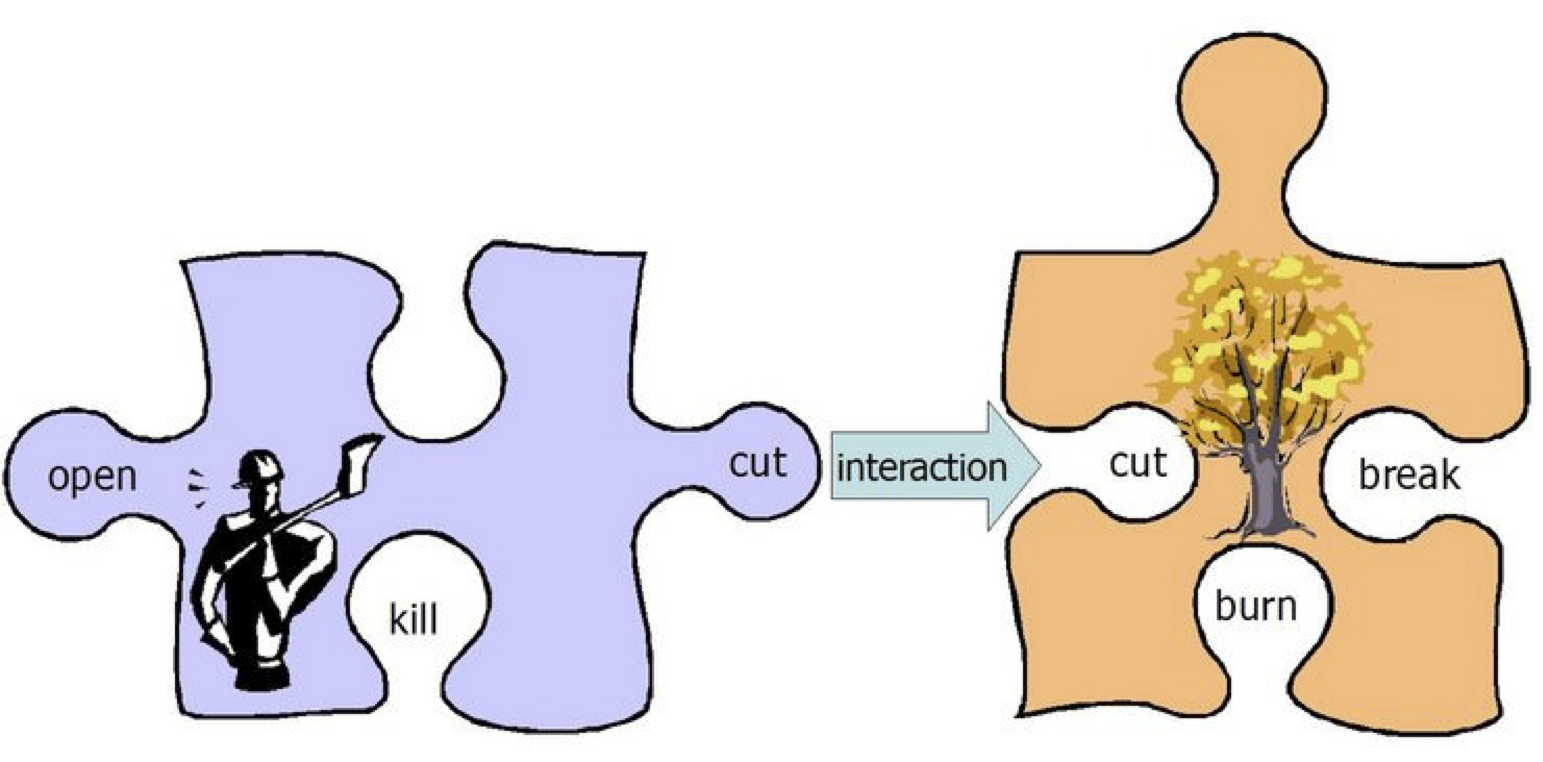
\includegraphics[scale=0.43]{img/moteur_ioda_explications.png}
\end{center}
\caption{Schéma récapitulatif quant au fonctionnement du moteur IODA.\\Deux agents sont présents : l'agent \textit{Woodcutter} et l'agent \textit{Tree}. Ce premier est doté de 3 interactions agissant chacune sur un agent : \textit{open}, \textit{kill}, \textit{cut} (sur un agent \textit{Tree}), tandis que le second détient de même 3 interactions qu'il subira : \textit{cut}, \textit{burn} et \textit{break}.\\Dans cette configuration, l'agent \textit{Woodcutter} n'a que l'agent \textit{Tree} parmi ses voisins - il préférera ainsi exécuter l'interaction \textit{cut}, après que les déclencheurs et conditions aient été validés.}
\label{fig:moteur_ioda_explications}
\end{figure}